% Préambule APMEP - Annales
% Auteurs
% tapuscrit : 			
% relecture :
% figures TikZ :
% figures pstricks :
% modifications :
% Remerciements :
% version 1
%
\documentclass[12pt,a4paper,french]{article}

% Packages
%%% codage et police utilisée
\usepackage[T1]{fontenc}
\RequirePackage{iftex}
\iftutex % moteur utf-8 lualatex, xelatex
	\usepackage{fourier-otf} % remplace fourier pour moteur utf8 (LuaLaTeX, XeLaTeX)
	% Alternatives nécéssite (LuaLaTeX, XeLaTeX)
    \usepackage{hyperref}
	%\usepackage{fontspec}% pour utiliser des fontes système
\else % pour les autres moteurs latex, pdflatex
	\usepackage[utf8]{inputenc}
	\usepackage{fourier}
	\usepackage{amsmath,amssymb}
    \usepackage[dvips]{hyperref}
    \renewcommand{\ttdefault}{lmtt}
\fi
\usepackage[normalem]{ulem}
\usepackage{pifont}
\usepackage{lscape}
% tableaux
\usepackage{multicol}
\usepackage{multirow}
\usepackage{tabularx}
\usepackage{tabularray}
% texte et composition
\usepackage{textcomp}
\usepackage{babel}
\usepackage[np]{numprint}
%
\usepackage{fancyhdr}
\usepackage{makeidx}
\makeindex
% pour le symbole €
\usepackage{eurosym}
\DeclareRobustCommand{\officialeuro}{%
  \ifmmode\expandafter\text\fi
  {\fontencoding{U}\fontfamily{eurosym}\selectfont e}}
\AtBeginDocument{\renewcommand{\euro}{\officialeuro}}
% couleurs étendues
\usepackage{xcolor}
% pour les listes
\usepackage{enumitem}
% Enumérations réglage par défaut
\setlist[itemize]{label=\textbullet,leftmargin=5mm,labelwidth=3mm,labelsep=2mm,align=left}
\setlist[enumerate]{labelindent=0pt, leftmargin=5mm, labelsep=2mm, labelwidth=3mm,labelsep=2mm, align= left}
\setlist[enumerate,1]{label = \textbf{\arabic*.}}
\setlist[enumerate,2]{label = \textbf{\alph*.}}
\setlist[enumerate,3]{label = \textbf{\roman*.}}
% pour l'ajustement des boites (figures…)
\usepackage{adjustbox}
% pour ne pas commencer un exercice en fin de page
\usepackage{needspace}
%
% Taille de la zone d'écriture
\usepackage[left=1.5cm,right=1.5cm,top=2.5cm,bottom=2.5cm]{geometry}
\setlength{\headheight}{15pt}
\setlength{\parindent}{0mm}
%
% Formatage du pdf
\hypersetup{%
    pdfauthor = {APMEP},
    pdfsubject = {Troisième, Série générale},
    pdftitle = {Brevet des collèges -- Métropole -- 10 septembre 2026},
    allbordercolors = white,
    pdfstartview=FitH
}
% Pour scratch (code)
\usepackage{scratch3}
% Pour le code Python
\usepackage{listings}
\lstdefinestyle{python}{
  language=Python,
  basicstyle=\ttfamily\small,
  keywordstyle=\color{blue}\bfseries,
  commentstyle=\color{gray}\itshape,
  stringstyle=\color{orange},
  numbers=left,
  numberstyle=\tiny\color{gray},
  breaklines=true,
  frame=single,
  backgroundcolor=\color{gray!5},
  tabsize=4
}
  % usage (exemple)
  %\begin{lstlisting}[style=python]
%def seuil():
%    n = 1
%    p = 0.5
%    while p < 0.6 :
%       n = n + 1
%       p = p*7/15 + 1/3
%    return n
%\end{lstlisting}


% Pour une visualisation de type tableur
\usepackage{pas-tableur}
%
%% pour PsTricks
\usepackage{pst-bezier}%% AVANT les autres PST
\usepackage{pstricks-add}
\usepackage{pst-func,pst-tree,pst-circ}
\usepackage{pst-eucl}
%% pour TikZ
\usepackage{tikz,pgfplots,pgf,tkz-tab,tikzpagenodes}
\usetikzlibrary{calc,patterns,decorations,arrows.meta,patterns.meta,arrows}
\pgfplotsset{compat=1.18,/pgf/number format/.cd,use comma}
\usepackage{icomma} % gestion des espaces autour des virgules
\DeclareMathSymbol{;}{\mathbin}{operators}{"3B}% pour un espacement correct du ; en mode maths
%%%%%%%%%%%%%%%%%%%%%%%%%%%%%%%%%%%%%%%%%%
% Définitions
%
% notation en mode mathématique et hors mode mathématique
\newcommand{\R}{\ensuremath{\mathbb{R}}}
\newcommand{\N}{\ensuremath{\mathbb{N}}}
\newcommand{\D}{\ensuremath{\mathbb{D}}}
\newcommand{\Z}{\ensuremath{\mathbb{Z}}}
\newcommand{\Q}{\ensuremath{\mathbb{Q}}}
\newcommand{\C}{\ensuremath{\mathbb{C}}}
%
\providecommand{\up}{\textsuperscript}
%
\newcommand{\vect}[1]{\overrightarrow{\,\mathstrut#1\,}}
\newcommand{\vectt}[1]{\overrightarrow{\,\mathstrut\text{#1}\,}}
%
\def\Oij{$\left(\text{O};\vect{\imath},\vect{\jmath}\right)$}
\def\Oijk{$\left(\text{O};\vect{\imath},\vect{\jmath},\vect{k}\right)$}
\def\Ouv{$\left(\text{O};\vect{u},\vect{v}\right)$}
%
\newcommand{\ds}{\displaystyle}
%
\renewcommand{\d}{\mathrm{\,d}}
\renewcommand{\i}{\mathrm{\,i\,}}
\newcommand{\e}{\mathrm{\,e\,}}
%%%%%%%%%%%%%%%%%%%%%%%%%%%%%%%%%%%%%%%%%%%

\begin{document}

%---------------------------------------------------------
% Réglage entête, pied de page
%---------------------------------------------------------
\rhead{\textbf{A. P{}. M. E. P{}.}}
\lhead{\small Sujet}
\lfoot{\small{Métropole -- Antilles -- Guyane}}
\rfoot{\small{10 septembre 2026}}
\pagestyle{fancy}

\thispagestyle{empty}


%---------------------------------------------------------
% Titre
%---------------------------------------------------------
\begin{center}
{\Large \textbf{
		\decofourleft~ Diplôme National du Brevet ~\decofourright\\[10pt]
		Série générale -- Métropole -- Antilles -- Guyane
		\marginpar{\rotatebox{90}{\textbf{A. P{}. M. E. P{}.}}}\\[10pt]
		 10 septembre 2026\\[10 pt]
		Sujet\\[10pt]}}
\end{center}

L'usage de la calculatrice avec mode examen actif ou sans mémoire \og type collège \fg{} est \textbf{interdit} pour la partie 1 et \textbf{autorisé} pour la partie 2.

L'utilisation du dictionnaire est interdite.

\bigskip

\section*{\centering PREMIÈRE PARTIE : AUTOMATISMES (6 pts)}

Pour chaque question, recopier sur la copie son numéro et la réponse correspondante.

Pour cette partie, aucune justification n'est demandée.

Pour les questions à choix multiple, une seule réponse est exacte.

\subsection*{Question 1}

Quelle est l'abscisse du point A ?

%Début Tikz
\begin{center}
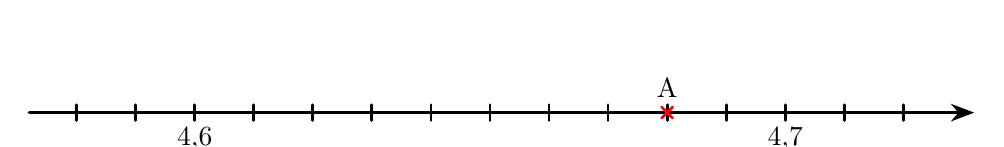
\begin{tikzpicture}[x=0.75cm,line cap=round, line join=round]
	\draw[line width=1.2pt,-{Stealth}] (-2.8,0) -- (13.2,0);
	\foreach \i in {-2,...,12} \draw[line width=1pt] (\i,-0.1) -- (\i,0.1);
	\node[below=2pt] at (0,0) {4,6};
	\node[below=2pt] at (10,0) {4,7};
	\draw[line width=1pt,red] (8,0) ++(2pt,2pt)--++(-4pt,-4pt) ++(0,4pt)--++(4pt,-4pt);
	\node[above=2pt] at (8,0) {A};
\end{tikzpicture}
\end{center}
%Fin Tikz

\subsection*{Question 2}

Quelle expression est égale à $4x+6x$ ?

\begin{center}
\begin{tblr}{*{4}{|X[c]}|}\hline
	\textbf{A.} $10x^2$ & \textbf{B.} $24x^2$ & \textbf{C.} $10x$ & \textbf{D.} $24x$ \\
	\hline
\end{tblr}
\end{center}

\subsection*{Question 3}

On tire au hasard une boule dans un sac et on sait que la probabilité d'obtenir une boule rouge est 0,4.

Quelle est la probabilité de ne pas obtenir une boule rouge ?

\subsection*{Question 4}

Une voiture part à 7~h 10~min. Le trajet dure 53~min.

À quelle heure arrive-t-elle ?

\subsection*{Question 5}

Le prix d'un objet est de 150~\euro. Il augmente de 10\,\%.

Quel est son nouveau prix ?

\begin{center}
\begin{tblr}{*{4}{|X[c]}|}\hline
	\textbf{A.} 135~\euro & \textbf{B.} 150,10~\euro & \textbf{C.} 160~\euro & \textbf{D.} 165~\euro \\
	\hline
\end{tblr}
\end{center}

\subsection*{Question 6}

Le graphique ci-dessous donne la taille d'une personne en fonction de son âge.

%Début Tikz
\begin{center}
		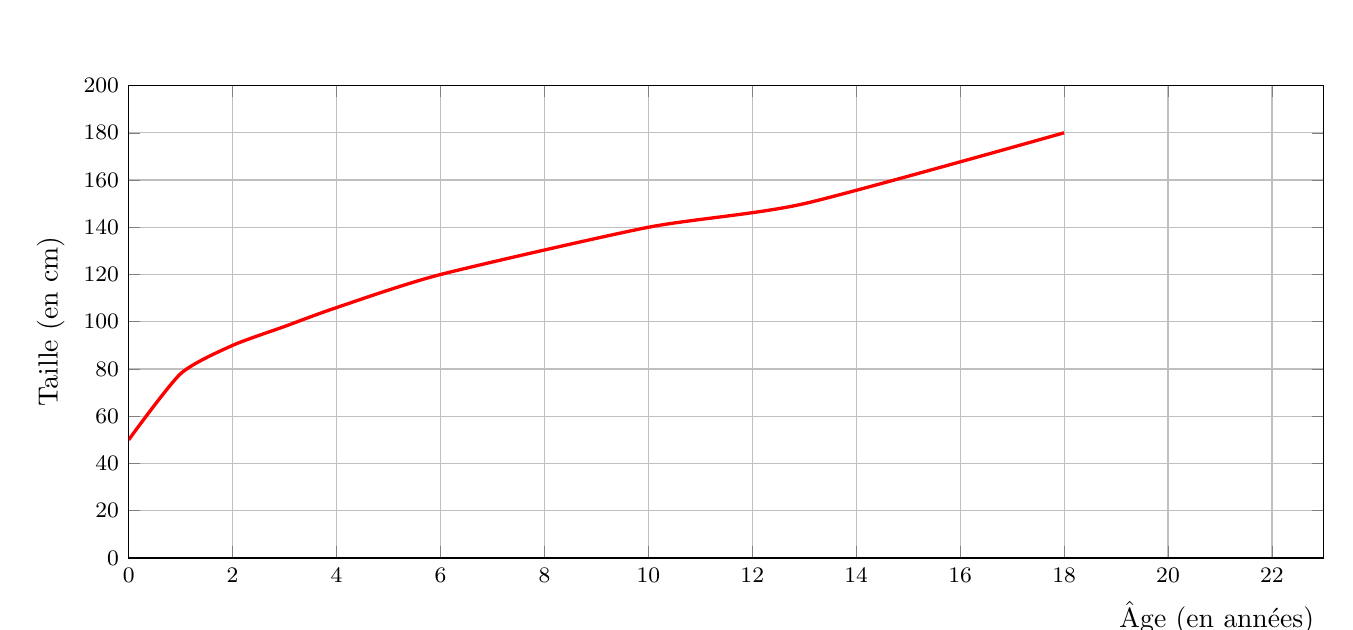
\begin{tikzpicture}%compiler avec pgfplots
			\begin{axis}[/pgf/number format/.cd, use comma,
				xlabel={Âge (en années)},
				xlabel style={
					at={(ticklabel cs:1)},
					anchor=north east},
				ylabel={Taille (en cm)},
				x={6.6mm}, y={0.3mm},
				xmin = 0, xmax = 23,
				ymin = 0, ymax = 200,
				xtick distance=2,
				ytick distance=20,
				tick label style={font=\footnotesize},
				grid=major]
				\addplot [line width=1.2pt,color=red,smooth,tension=0.4] coordinates
					{(0,50) (1,78) (2,90) (3,98) (4,106) (6,120) (10,140) (13,150) (18,180)};
			\end{axis}
		\end{tikzpicture}
\end{center}
%Fin Tikz

À partir de quel âge la taille de cette personne a-t-elle dépassé 140~cm ?

\subsection*{Question 7}

Parmi les nombres ci-dessous, lequel est divisible par 3 ?

\begin{center}
\begin{tblr}{*{4}{|X[c]}|}\hline
	\textbf{A.} 307 & \textbf{B.} 954 & \textbf{C.} \np{1201} & \textbf{D.} \np{22003} \\
	\hline
\end{tblr}
\end{center}

\begin{minipage}{0.52\linewidth}
\subsection*{Question 8}

La figure ci-contre n'est pas représentée en vraie grandeur.

Quelle est la mesure de l'angle $\widehat{\mathrm{BAC}}$ ?

\medskip

\begin{tblr}{*{2}{|X[c]}|}\hline
	\textbf{A.} 80\degres & \textbf{B.} 90\degres \\ \hline
	\textbf{C.} 100\degres & \textbf{D.} 110\degres \\ \hline
\end{tblr}
\end{minipage}\hfill
%Début Tikz
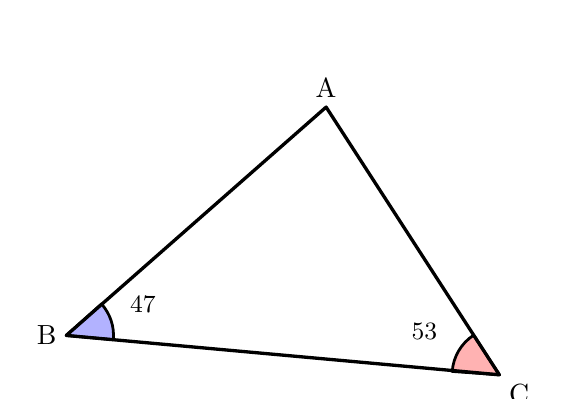
\begin{tikzpicture}[line cap=round, line join=round,baseline={(current bounding box.center)}]
	\coordinate (B) at (0,0);
	\coordinate (C) at (5.5,-0.5);
	\coordinate (A) at (3.3,2.9);
	\draw[line width=1pt,fill=blue!30] (B) -- ($(B)!0.6cm!(C)$) arc[start angle={atan2(-0.5,5.5)}, delta angle=47, radius=0.6cm] -- cycle;
	\draw[line width=1pt,fill=red!30] (C) -- ($(C)!0.6cm!(A)$) arc[start angle={atan2(3.4,-2.2)}, delta angle=53, radius=0.6cm] -- cycle;
	\draw[line width=1.2pt] (A) -- (B) -- (C) -- cycle;
	\node[font=\small] at ($(B)+(22:1.05)$) {47\degres};
	\node[font=\small] at ($(C)+(150:1.1)$) {53\degres};
	\node[above] at (A) {A};
	\node[left] at (B) {B};
	\node[below right] at (C) {C};
\end{tikzpicture}\hfill~
%Fin Tikz

\subsection*{Question 9}

Quel est le résultat de $\dfrac{5}{8} \div \dfrac{8}{9}$ ?

\begin{center}
\begin{tblr}{*{4}{|X[c]}|}\hline
	\textbf{A.~~} $\dfrac{45}{64}$ & \textbf{B.~~} $\dfrac{45}{8}$ & \textbf{C.~~} $\dfrac{40}{72}$ & \textbf{D.~~} $\dfrac{5}{9}$ \\
	\hline
\end{tblr}
\end{center}

\begin{center}
\emph{Restitution de la copie du candidat à l'issue de la partie $1$}
\end{center}

\newpage

\section*{\centering DEUXIÈME PARTIE (14 pts)}

\begin{quote}
\emph{Dans cette partie, toutes les réponses doivent être justifiées, sauf si une indication contraire est donnée.\\
	La clarté et la précision des raisonnements ainsi que la rédaction sont évaluées sur 2 points.\\
	Pour chaque question, si le travail n'est pas terminé, laisser tout de même une trace de la recherche ; les essais et les démarches engagées, même non aboutis, seront pris en compte dans la notation.}
\end{quote}

\needspace{10\baselineskip}
\section*{Exercice 1 \hfill 3,5 points}

\emph{Les parties {\rm A} et {\rm B} de cet exercice sont indépendantes.}

\medskip

Le tableau ci-dessous donne le nombre total de médailles obtenues par 3 nations européennes, l'Italie, la France et la Norvège, lors de six éditions des Jeux Olympiques d'hiver.

\begin{center}
\begin{tblr}{colspec={|X[c]|*{6}{X[c]|}},row{1}={font=\bfseries},column{1}={font=\bfseries}}
	\hline
	Médailles & 2002 & 2006 & 2010 & 2014 & 2018 & 2022 \\ \hline
	Italie    & 13   & 11   & 5    & 8    & 10   & 17   \\ \hline
	France    & 11   & 9    & 11   & 15   & 15   & 14   \\ \hline
	Norvège   & 25   & 19   & 23   & 27   & 39   & 37   \\ \hline
\end{tblr}
\end{center}

\subsection*{Partie A}

\begin{enumerate}
	\item Donner le nombre de médailles obtenues par la France en 2010.
	\item Calculer la moyenne des médailles obtenues par la France lors de ces 6 jeux olympiques.
	\item Lors des jeux olympiques de 2002, la Norvège a terminé à la première place des nations. Elle avait obtenu au total 25 médailles dont 13 médailles en or.

	Calculer le pourcentage de médailles d'or gagnées par la Norvège en 2002 par rapport au nombre total des médailles qu'elle a obtenues cette année-là.
\end{enumerate}

\subsection*{Partie B}

Pour accéder au point de départ d'une épreuve, les skieurs utilisent un téléphérique dont le schéma ci-dessous représente le déplacement entre les points A et B.

%Début Tikz
\begin{center}
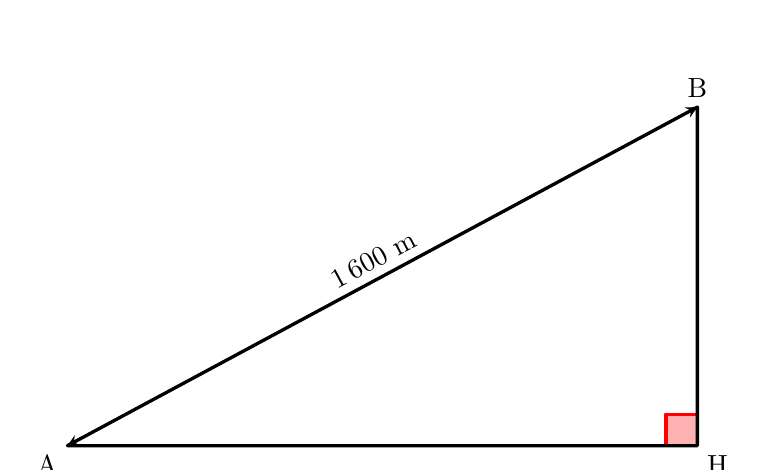
\begin{tikzpicture}[line cap=round, line join=round]
	\coordinate (A) at (0,0);
	\coordinate (H) at (8,0);
	\coordinate (B) at (8,4.3);
	\draw[line width=1.2pt,red,fill=red!30] (H) rectangle ++(-0.4,0.4);
	\draw[line width=1.2pt] (A) -- (H) -- (B) -- cycle;
	\node[below left] at (A) {A};
	\node[below right] at (H) {H};
	\node[above] at (B) {B};
	\draw[<->, line width=0.8pt, > = stealth,shift={(118.26:0.5)}] (A) -- (B) node[pos=0.5,above,sloped]{\np{1600}~m};
\end{tikzpicture}
\end{center}
%Fin Tikz

La longueur AB est égale à \np{1600}~m.

L'altitude du point A est \np{1814}~m et celle du point B est \np{2359}~m.

Les points A et H sont à la même altitude.

\begin{enumerate}
	\item Montrer que la différence d'altitude entre les points H et B, c'est-à-dire la longueur HB, est égale à 545~m.
	\item Pour respecter les normes de sécurité du téléphérique, la mesure de l'angle $\widehat{\mathrm{BAH}}$ doit être inférieure à 30\degres.

	Cette norme est-elle respectée ?\\
	\textbf{Détailler la réponse en précisant la démarche.}
	\item La vitesse du téléphérique est égale à 5~m/s.

	Quelle est la durée du trajet entre A et B ? Donner le résultat en minutes et secondes.
\end{enumerate}

\needspace{10\baselineskip}
\section*{Exercice 2 \hfill 4 points}

Le schéma ci-dessous représente un terrain SMVU. Il n'est pas à l'échelle.

%Début Tikz
\begin{center}
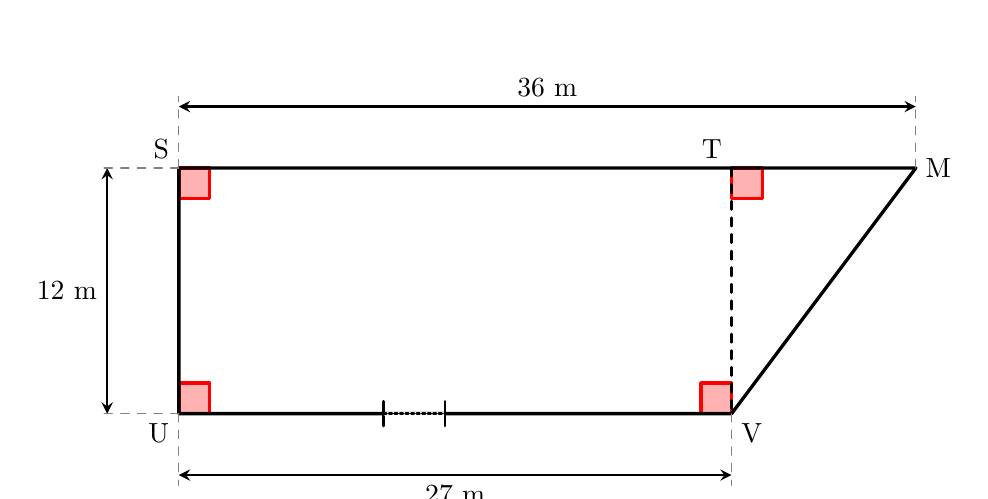
\begin{tikzpicture}[x=0.26cm,y=0.26cm,line cap=round, line join=round]
	\coordinate (S) at (0,12);
	\coordinate (T) at (27,12);
	\coordinate (M) at (36,12);
	\coordinate (U) at (0,0);
	\coordinate (V) at (27,0);
	% angles droits
	\draw[line width=1.2pt,red,fill=red!30]
		(S) rectangle ++(1.5,-1.5)
		(T) rectangle ++(1.5,-1.5)
		(U) rectangle ++(1.5,1.5)
		(V) rectangle ++(-1.5,1.5);
	\draw[line width=1.2pt] (U) -- (S) -- (M) -- (V) -- cycle;
	\draw[line width=1pt,dashed] (T) -- (V);
	% ouverture du portail
	\draw[line width=1pt] (10,-0.6) -- (10,0.6) (13,-0.6) -- (13,0.6);
	\draw[line width=1.5pt,white] (10.1,0) -- (12.9,0);
	\draw[line width=1pt,densely dotted] (10,0) -- (13,0);
	% cotes
	\draw[<->, line width=0.8pt, > = stealth] (0,15) -- (36,15) node[pos=0.5,above]{36 m};
	\draw[<->, line width=0.8pt, > = stealth] (-3.5,0) -- (-3.5,12) node[pos=0.5,left]{12 m};
	\draw[<->, line width=0.8pt, > = stealth] (0,-3) -- (27,-3) node[pos=0.5,below]{27 m};
	\draw[line width=0.4pt,gray,dashed] (0,12) -- (0,15.5) (36,12) -- (36,15.5)
		(0,12) -- (-4,12) (0,0) -- (-4,0)
		(0,0) -- (0,-3.5) (27,0) -- (27,-3.5);
	\node[above left] at (S) {S};
	\node[above left] at (T) {T};
	\node[right] at (M) {M};
	\node[below left] at (U) {U};
	\node[below right] at (V) {V};
\end{tikzpicture}
\end{center}
%Fin Tikz

On souhaite poser du gazon sur la partie rectangulaire STVU et cultiver un potager sur la partie triangulaire TMV.

On désire également clôturer ce terrain SMVU avec du grillage en laissant une ouverture de 3~m pour le futur portail qui sera placé sur le côté [UV].

\begin{enumerate}
	\item Justifier que la longueur TM est égale à 9~m.
	\item Montrer que la longueur MV est égale à 15~m.
	\item Quelle longueur de grillage doit-on prévoir ?
	\item Montrer que la surface de la partie du terrain STVU recouverte de gazon est égale à 324~m$^2$.
	\item Le cadre ci-dessous donne les informations que l'on peut lire sur l'étiquette d'un rouleau de gazon.

	\begin{center}
	\begin{tblr}{colspec={|l|},row{1}={font=\bfseries,halign=c}}
		\hline
		Caractéristiques d'un rouleau une fois déroulé \\
		Forme : rectangulaire \\
		Longueur : 4~m \\
		Largeur : 2~m \\
		Épaisseur : 30~mm \\
		Prix : 86~\euro \\ \hline
	\end{tblr}
	\end{center}

	On veut recouvrir de gazon le rectangle STVU.

	Un budget de \np{3500}~\euro{} est-il suffisant ?\\
	\textbf{Détailler la réponse en précisant la démarche.}
\end{enumerate}

\needspace{10\baselineskip}
\section*{Exercice 3 \hfill 4,5 points}

On considère les deux programmes de calcul suivants.

\begin{center}
	\fbox{\begin{minipage}[t]{0.4\textwidth}
		{\centering \textbf{Programme A}\par}
		\begin{itemize}[nosep]
			\item Choisir un nombre.
			\item Lui ajouter 3.
			\item Calculer le carré de la somme obtenue.
			\item Soustraire 9 au résultat.
		\end{itemize}
	\end{minipage}}
	\hfill
	\fbox{\begin{minipage}[t]{0.48\textwidth}
		{\centering \textbf{Programme B}\par}
		\begin{itemize}[nosep]
			\item Choisir un nombre.
			\item Lui ajouter 6.
			\item Multiplier le résultat obtenu par le nombre de départ.
		\end{itemize}
	\end{minipage}}
\end{center}

\begin{enumerate}
	\item On choisit 4 comme nombre de départ.
	\begin{enumerate}
		\item Montrer qu'on obtient 40 avec le programme A.
		\item Quel résultat obtient-on avec le programme B ?
	\end{enumerate}
	\item On utilise un tableur pour obtenir d'autres résultats.

	\begin{center}
	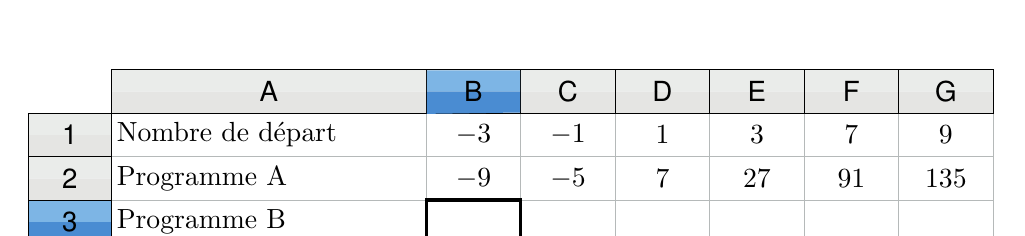
\begin{tikzpicture}
		\tableur*[3]{A/4cm,B/1.2cm,C/1.2cm,D/1.2cm,E/1.2cm,F/1.2cm,G/1.2cm}
		\celtxt[width=4cm]{A}{1}{Nombre de départ}
		\celtxt[width=4cm]{A}{2}{Programme A}
		\celtxt[width=4cm]{A}{3}{Programme B}
		\celtxt*[width=1.2cm,align=center]{B}{1}{$-3$}
		\celtxt*[width=1.2cm,align=center]{C}{1}{$-1$}
		\celtxt[width=1.2cm,align=center]{D}{1}{1}
		\celtxt[width=1.2cm,align=center]{E}{1}{3}
		\celtxt[width=1.2cm,align=center]{F}{1}{7}
		\celtxt[width=1.2cm,align=center]{G}{1}{9}
		\celtxt*[width=1.2cm,align=center]{B}{2}{$-9$}
		\celtxt*[width=1.2cm,align=center]{C}{2}{$-5$}
		\celtxt[width=1.2cm,align=center]{D}{2}{7}
		\celtxt[width=1.2cm,align=center]{E}{2}{27}
		\celtxt[width=1.2cm,align=center]{F}{2}{91}
		\celtxt[width=1.2cm,align=center]{G}{2}{135}
		\selecCell{B}{3}
	\end{tikzpicture}
	\end{center}

	Quelle formule doit-on saisir dans la cellule B3 afin qu'elle soit étirée vers la droite pour compléter le tableau ?
\end{enumerate}

\begin{minipage}[t]{0.52\linewidth}
\begin{enumerate}[start=3]
	\item Soit $f$ la fonction qui, à un nombre de départ $x$, associe le nombre obtenu par le programme B. La courbe ci-contre représente la fonction $f$.
	\begin{enumerate}
		\item Déterminer graphiquement l'image de $-3$ par la fonction $f$.
		\item Déterminer graphiquement les antécédents de $-5$ par la fonction $f$.
	\end{enumerate}
	\item Déterminer par le calcul tous les nombres permettant d'obtenir 0 par le programme B.
	\item On désigne par $x$ le nombre choisi au départ.
	\begin{enumerate}
		\item Démontrer que : $(x + 3)(x + 3) = x^2 + 6x + 9$.
		\item Montrer que les deux programmes donnent le même résultat quel que soit le nombre $x$ choisi au départ.
	\end{enumerate}
\end{enumerate}
\end{minipage}\hfill
\begin{minipage}[t]{0.44\linewidth}
\vspace{0pt}
%Début Tikz
\begin{center}
	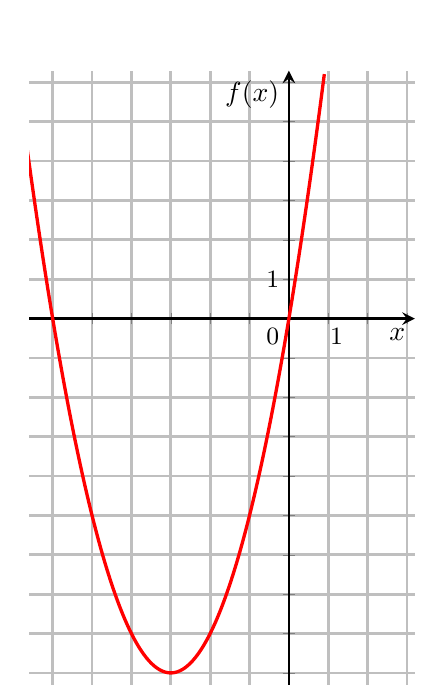
\begin{tikzpicture}%compiler avec pgfplots
		\begin{axis}[axis lines=middle,
			x={5mm}, y={5mm},
			xmin = -6.6, xmax = 3.2,
			ymin = -9.6, ymax = 6.3,
			xtick = {-6,...,3}, ytick = {-9,...,6},
			xticklabels = {}, yticklabels = {},
			grid=major,
			grid style={line width=1pt,gray!50},
			xlabel={$x$}, ylabel={$f(x)$},
			xlabel style={anchor=north east},
			ylabel style={anchor=north east},
			>=stealth, axis line style={line width=1pt,->}]
			\addplot [line width=1.2pt,color=red,smooth,samples=120,domain=-6.9:0.9]{x^2+6*x};
			\node[below right,font=\small] at (axis cs:0.8,0) {1};
			\node[left,font=\small] at (axis cs:0,1) {1};
			\node[below left,font=\small] at (axis cs:0,0) {0};
		\end{axis}
	\end{tikzpicture}
\end{center}
%Fin Tikz
\end{minipage}

\end{document}
